\documentclass{standalone}
\usepackage{tikz}

\usetikzlibrary{calc}


\begin{document}

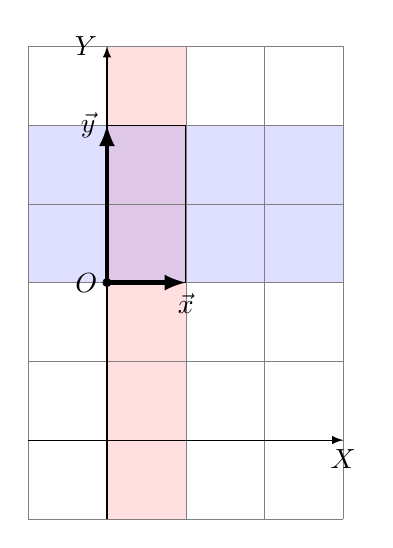
\begin{tikzpicture}
  \path[fill=red!50,opacity=.25] (0,-1) rectangle (1,5);
  \path[fill=blue!50,opacity=.25] (-1,2) rectangle (3,4);
  \draw[ultra thin,gray] (-1,-1) grid (3,5);
  \draw[-latex] (-1,0) -- (3,0) node[below] {$X$};
  \draw[-latex] (0,-1) -- (0,5) node[left] {$Y$};
  \draw (0,2) rectangle (1,4);

  \draw[fill] (0,2) circle[radius=0.05] node[left] {$O$};
  \draw[-latex,ultra thick] (0,2) -- ++(1,0) node[below] {$\vec{x}$};
  \draw[-latex,ultra thick] (0,2) -- ++(0,2) node[left] {$\vec{y}$};
\end{tikzpicture}

\end{document}